\documentclass[letterpaper,12pt]{article}
\usepackage[margin=1in]{geometry}
\usepackage{xltxtra}
\setmainfont[Mapping=tex-text]{Liberation Serif}
\setmonofont[Scale=0.8]{Liberation Mono}
\newcommand{\var}[1]{\texttt{\$\{#1\}}}
\usepackage[colorlinks=false,pdfborder=0 0 0]{hyperref}
\usepackage{graphicx}
\usepackage[numbib]{tocbibind}

\title{Instalog Project Report \\
Interim Report 2}
\author{
Billy R. O'Neal III (bro4@case.edu) \\
Jacob Snyder (jrs213@case.edu) \\ \\
Case Western Reserve University
}

\begin{document}

\maketitle
\vspace{1in}
\begin{center}

\includegraphics[width=2in, height=2in]{figures/InstalogLogo.png}
\end{center}
\newpage



\tableofcontents
\newpage



\section{Abstract} \label{abstract}
The Microsoft Windows operating system is a complicated system.  When it is
working, everything is fine.  However, when something goes wrong, it is often a
frustrating experience troubleshooting what the problem is, so frequently the
easiest fix is to backup the machine and then reformat it and reinstall Windows.
This approach can severely impact productivity and is complicated for
non-technical users.  

One common source of problems for users of the Windows operating system is
infection from malware.  This has caused there to be a sizable market for
antimalware software.  This software is very effective at removing common
infections because at a high level, the software vendors simply need to maintain
a list of common infections and the safe way to remove them.  Some tools are
even moderately effective at removing unknown threats by using heuristic
techniques.  However, these techniques have limited effectiveness especially
against obscure or new malware.  

Therefore, a demand exists for tools that aid users in removing these obscure
malware infections.  This project, Instalog, is a response to this need. 
Instalog is designed to be a tool with two purposes: information gathering and
system repair.

First, it scans Windows installations to gather as much information as possible
about the machine.  It then filters this information using whitelists to remove
mundane information like system defaults.  It outputs a log of information that
is non-standard on the machine which will hopefully aid an expert in identifying
what the root cause of an infection is.

Second, Instalog provides a capacity to fix infections.  Given a log output,
experts can generate scripts to fix an infection either by hand or by using the
GUI.  Instalog can run these scripts to remove an infection.  

Instalog is designed such that it can support three different ``user classes.'' 
The first is that of a ``home user'' that has an infected machine but doesn't
know how to fix it.  This user can use Instalog to scan their machine and then
post it online to get assistance.  Here, an ``expert'' can download the ``home
user's'' log, analyze it, and produce a fix script for them to run.  The ``home
user'' can then download this script and run it using Instalog to fix their
machine.  This process may involve several iterations.  The other user case is
that of a ``system administrator'' that plays both roles -- ``system
administrators'' use Instalog to scan their machines and know enough about the
machine to generate and run a suitable fix script.  

\newpage



\section{Introduction} \label{introduction}
\subsection{Background}
There most certainly is a real need for this product.  In the Related Work
section before, other similar products are listed.  However, they all have their
associated problems and have not been maintained.  There are security
communities online such as Malware Bytes that use these tools to analyze and fix
users' machines.  These forums serve thousands of people a year, and the tools
are downloaded even more frequently after year.  Once this tool is fully
developed, the hope is that this will become the de-facto standard and replace
other tools.

\subsection{Related Work}
Instalog is inspired by several similar tools which all share some basic
functionality.  In many ways, Instalog can be viewed as an evolution of
these tools:

\begin{itemize}
    \item TrendMicro's {\em Hijack This} (HJT)
    \item ``sUBs'' {\em Doesn't Do Squat} (DDS)
    \item ``random/random'''s {\em Random's System Information Tool} (RSIT)
    \item ``OldTimer'''s {\em OTA}, {\em OTS}, and {\em OTL} (formerly
    OTAnalyzeIt, OTScanIt, and OTListIt, respectively)
    \item Sysinternals' {\em Autoruns}
    \item Runscanner's {\em Runscanner}
\end{itemize}

All of these tools purport to accomplish similar goals to Instalog. However,
each of these tools has bugs or specific behavior which cause problems for at
least one of Instalog's three intended user groups.  Specifically, the above
tools contain one or more of the above problems:

\begin{itemize}
    \item Incorrect handling and escaping of log data
    \item Lack of published specifications, documentation, or source code
    \item Outstanding bugs that the authors are unwilling or unable to fix
    \item Lack of scriptability, for the purposes of modifying log output and
    malware removal.
    \item Lack of 64 bit support.
    \item Lack of Unicode support.
    \item Lack of enumeration of some types of useful log information.
\end{itemize}

Instalog will attempt to solve those problems by combining characteristics of
the above tools which are deemed useful while mixing in a few tricks of its
own.

TrendMicro's {\em Hijack This} was open-sourced recently.  The authors of this
project have briefly looked through the project to see if it is worth forking
the project to implement Instalog.  It was determined that the source code is
not up to par.  Not only is it written in Visual Basic, the licensing agreement
on it is unknown at this time.  

\subsection{Progress}
At the time of the last report, we had finished the requirements and
specifications documents and had just started the design and code implementation
phase.  By working long hours over spring break, we have finished the design for
the scanning portion of the project and have moved into the implementation
phase.  So far, we have finished most of the background scaffolding needed to do
scanning (registry enumeration, filesystem enumeration, string manipulation,
etc.) and have moved into the actual implementation of the scanning section. 
With the exception of whitelisting, the running processes and scanners/drivers
sections are complete.  At the time of this writing, progress into Pseudo HJT
and Restore Point enumeration has begun.  

At this time, support for Windows 2000, Windows XP RTM, and Windows XP Service
Pack 1 have been tentatively dropped. This is forced upon us by changes made to
the C runtime bundled with Visual Studio 2010 which drops support for these
operating systems. (The application crashes on startup) We are actively
investigating workarounds for the problem.

Please refer to section~\ref{project_progress} for more details.  

\subsection{Report Structure}
This report is structured using a modified version of the structure proposed in
\cite{ReportGuidelines}.

This report begins with the proposed Abstract (section~\ref{abstract}),
Introduction (section~\ref{introduction}), and Application
(section~\ref{application}) sections.  The Methodology section is not an
explicit section in this document as it has been integrated into the other
documentation of the project.  Therefore, the report dives straight into the
heart of the documentation of the project in the Software Design section
(section~\ref{software_design}).  Since the documentation for this project is
extremely long, this section simply introduces the documents and references them
as external documents.  The proposed User Interface section has been included in
the documents listed in the Software Design section.  Similarly, the proposed
Testing and Evaluation section has been merged into the Software Design section
as a separate stand-alone document. This report then introduces the
aforementioned Scope Limit (section~\ref{scope_limit}) and then moves into the
finer points of the Project Management and Administrative Details
(section~\ref{project_management}) and Project Progress
(section~\ref{project_progress}) sections.  The report then references any
additional external documents in the External Documents section
(section~\ref{documents}) and then lists all of the references made in the
document in the References section.  Lastly, the report mentions the legal
details for the project in the License appendix (appendix~\ref{license}).

\newpage



\section{Application} \label{application}
Instalog can be seen as having three different distinct components:

\begin{enumerate}
  \item Scanning
  \item Scripting and Repairing
  \item GUI
\end{enumerate}

Each of these components will be expanded on in the following subsections.

\subsection{Scanning}
Instalog's scanning abilities are the information-gathering and whitelist
capabilities that will be provided to the user.  Instalog will scan a number of
different types of information such as registry keys, browser settings, and
recently modified files.  These different information points are picked because
they are primarily ``loading points,'' that is, they are locations that malware
would need to modify to be loaded.  Each information point will be filtered
using whitelists that will remove default values and values that are known to be
safe.  What will be left is information that is unique to the user's computer,
hopefully some of which provides information about the malware.

A big challenge with this is the sheer amount of data that is being included in
the scan.  The Instalog project team plan on getting around this by writing
meticulously detailed requirements and specifications documents to make sure
each behavior is well defined before starting to implement the project.
Another challenge with this is making the scan run quickly.  The biggest
challenge is to simply test the scanning behavior.  Since it is impossible to
anticipate every possible machine configuration, the software must be robust
enough to handle varying scenarios across all of the targeted versions of
Windows.

\subsection{Scripting and Repairing}
The next component is Instalog's ability to run scripts and repair systems. 
Instalog will define a scripting language that enables common actions such as
process killing, registry actions, and file quarantine.  It will also provide
scripting actions to run all of the available scanning actions.  This will allow
a script to gather more information about a system if necessary.  

The biggest challenge to this is similar to the scanning challenge -- it will be
very difficult to thoroughly test this.  It is \textit{imperative} that this
functionality is tested extensively though because one mistake in this component
could lead to data loss on a user's machine.  

\subsection{GUI}
The final component of Instalog is the graphical user interface (GUI).  This
interface will allow users to run scans, run scripts, and build scripts based on
scan outputs.  The challenge here is building the GUI using the native GUI
controls, especially since some of the proposed screens such as the script
builder are incredibly complex.  Additionally, the script builder must be tested
heavily as well, because if a poor script is built, this could also lead to data
loss on a user's machine.  

\newpage



\section{Software Design} \label{design}
The nature of this tool is that there are a lot of small little features that
collectively make up each component mentioned in the Application section
(section~\ref{application}).  Alone, each small feature of the tool is quite
manageable and straightforward.  However, when all of the pieces are put
together, there is actually an impressive amount of detail and small nuances
that are required to adequately explain each feature.  Therefore, instead of
including the Software Requirements, Software Specifications, Software Design,
and Testing and Validation documents in this report, they have been written and
included as stand-alone documents.  This was done with the intent of making this
document more readable as well as making each document more maintainable when
they inevitably have to be updated or modified throughout the product
development lifecycle.  Each document is briefly introduced, explained, and
referenced in the following subsections.  Please refer to the specified
documents for more details.

\subsection{Software Requirements}
\label{software_requirements}
The Software Requirements document \cite{Requirements} is designed to be read by
a mostly non-technical audience.  It describes the various features that the
project will have and what criteria these features must meet to be considered
implemented successfully.  This document is written at a fairly high-level view
as the problem space is fairly well defined for this project.

\subsection{Software Requirements Specifications}
\label{software_specifications}
The Software Requirements Specifications document \cite{Specification} is the
document that visits each requirement in the above Software Requirements
document.  This document is quite long because it describes in meticulous detail
how each feature will function, how it must behave, where the data will be
pulled from, etc.  The intent of this document is that it will make the actual
design, implementation, and testing of the project much easier because the
behavior is well defined from the start.  This document has also been released
in private security volunteer circles for validation, and has been modified
slightly at the suggestions of a few individuals.

\subsection{Software Design}
\label{software_design}
The Design document \cite{Design} is the document that describes how the
requirements will be implemented.  This document is currently a work in progress
and explains the progress made and current plan for remaining items.  Please
note that it does \textit{not} attempt to document the features that are not
part of the scope limit.  This being said, however, it does have some plans made
for things such as scripting and user interfaces.  

\subsection{Testing and Validation}
\label{testing_and_evaluation}
The Testing and Validation document \cite{Testing} is the document that
describes how the tool will be evaluated.  Since the Requirements
Document \cite{Requirements} and Software Requirements Specification
\cite{Specification} document describe each facet of the tool in extreme
detail, the expected behavior of the tool must just match the requirements.  The
Testing and Validation document is a brief document that describes the approach
in the project to testing, specifically unit testing.  It will be updated as the
project progresses to reflect the integration and system testing that will be
done once more of the project is completed.

\newpage



\section{Scope Limit} \label{scope_limit}
The scope of this project is much larger than can be reasonably finished in the
time-frame for the course.  It has taken five weeks just to write the
requirements and specifications for the project.  Therefore, due to the sheer
amount of features this tool will have as well as the amount of testing on
varying environments that will be required, at the suggestion of the professor
of the Senior Project course, the authors have instituted a scope limit for the
completion of the project.  Since the scanning functionality is the most
valuable part of the tool, this functionality will be completed in time for the
project deadline of the course.  If this functionality is completed and verified
quickly and there is time to spare, the following features will be added in the
specified order:

\begin{enumerate}
    \item Scripting 
    \item GUI 
    \item Enumeration of Firefox data
    \item Enumeration of Google Chrome data
    \item Spoofed DNS check
    \item ``Value Added'' scripting actions, such as MRC upload or VirusTotal
    upload
    \item Checkboxes and fix generation on the GUI
\end{enumerate}

In the event any of these features are added, Instalog will remain a functional,
shippable, well-tested, production-quality tool, suitable for the final senior
project submission.  If a feature is attempted but cannot be developed to a
satisfactory level in time for the submission, a previously stable release of
the tool will be reverted to and turned in.  

The authors of this tool will complete any remaining deliverables outside of the
Senior Project course in the free time between when classes and summer
internships / employment begins.  

\newpage



\section{Project Management and Administrative Details}
\label{project_management} 
When the concept for this project was originally realized, the intent was that
the entire project would be implemented, tested, and shippable by the end of the
Senior Project class.  However, since the authors have other courses as well as
jobs and extra-curricular activities, it gradually became evident that the
original timeline would not be even remotely feasible.  For instance, the
original hope was the entire Software Requirements Specification
\cite{Specification} would be finished in a day over the weekend.  Despite
working on the document for an entire weekend, the document was not finished in
the intended time period.  In fact, it took several weeks to finish the
document.  

Around the due date of the Project Proposal, the authors spent some time
developing a realistic view of the project.  Out of this came the Scope Limit
(section~\ref{scope_limit}) explained in the preceding section.  It was decided
that instead of letting standards slip and shipping a shoddy product that could
potentially ruin users' machines, that instead the first component of the
product would be implemented and tested well.  Then, after the course, work
would continue on the remaining items.  The hope is that since the Specification
Document was written so thoroughly, the implementation and testing will not be
as time consuming and that the timeline can be shortened and more features can
be implemented.  However, given the oversights that were present in the original
timeline, this is the best realistic timeline that is possible at the moment.  

\begin{figure}[h]
  	\centering
	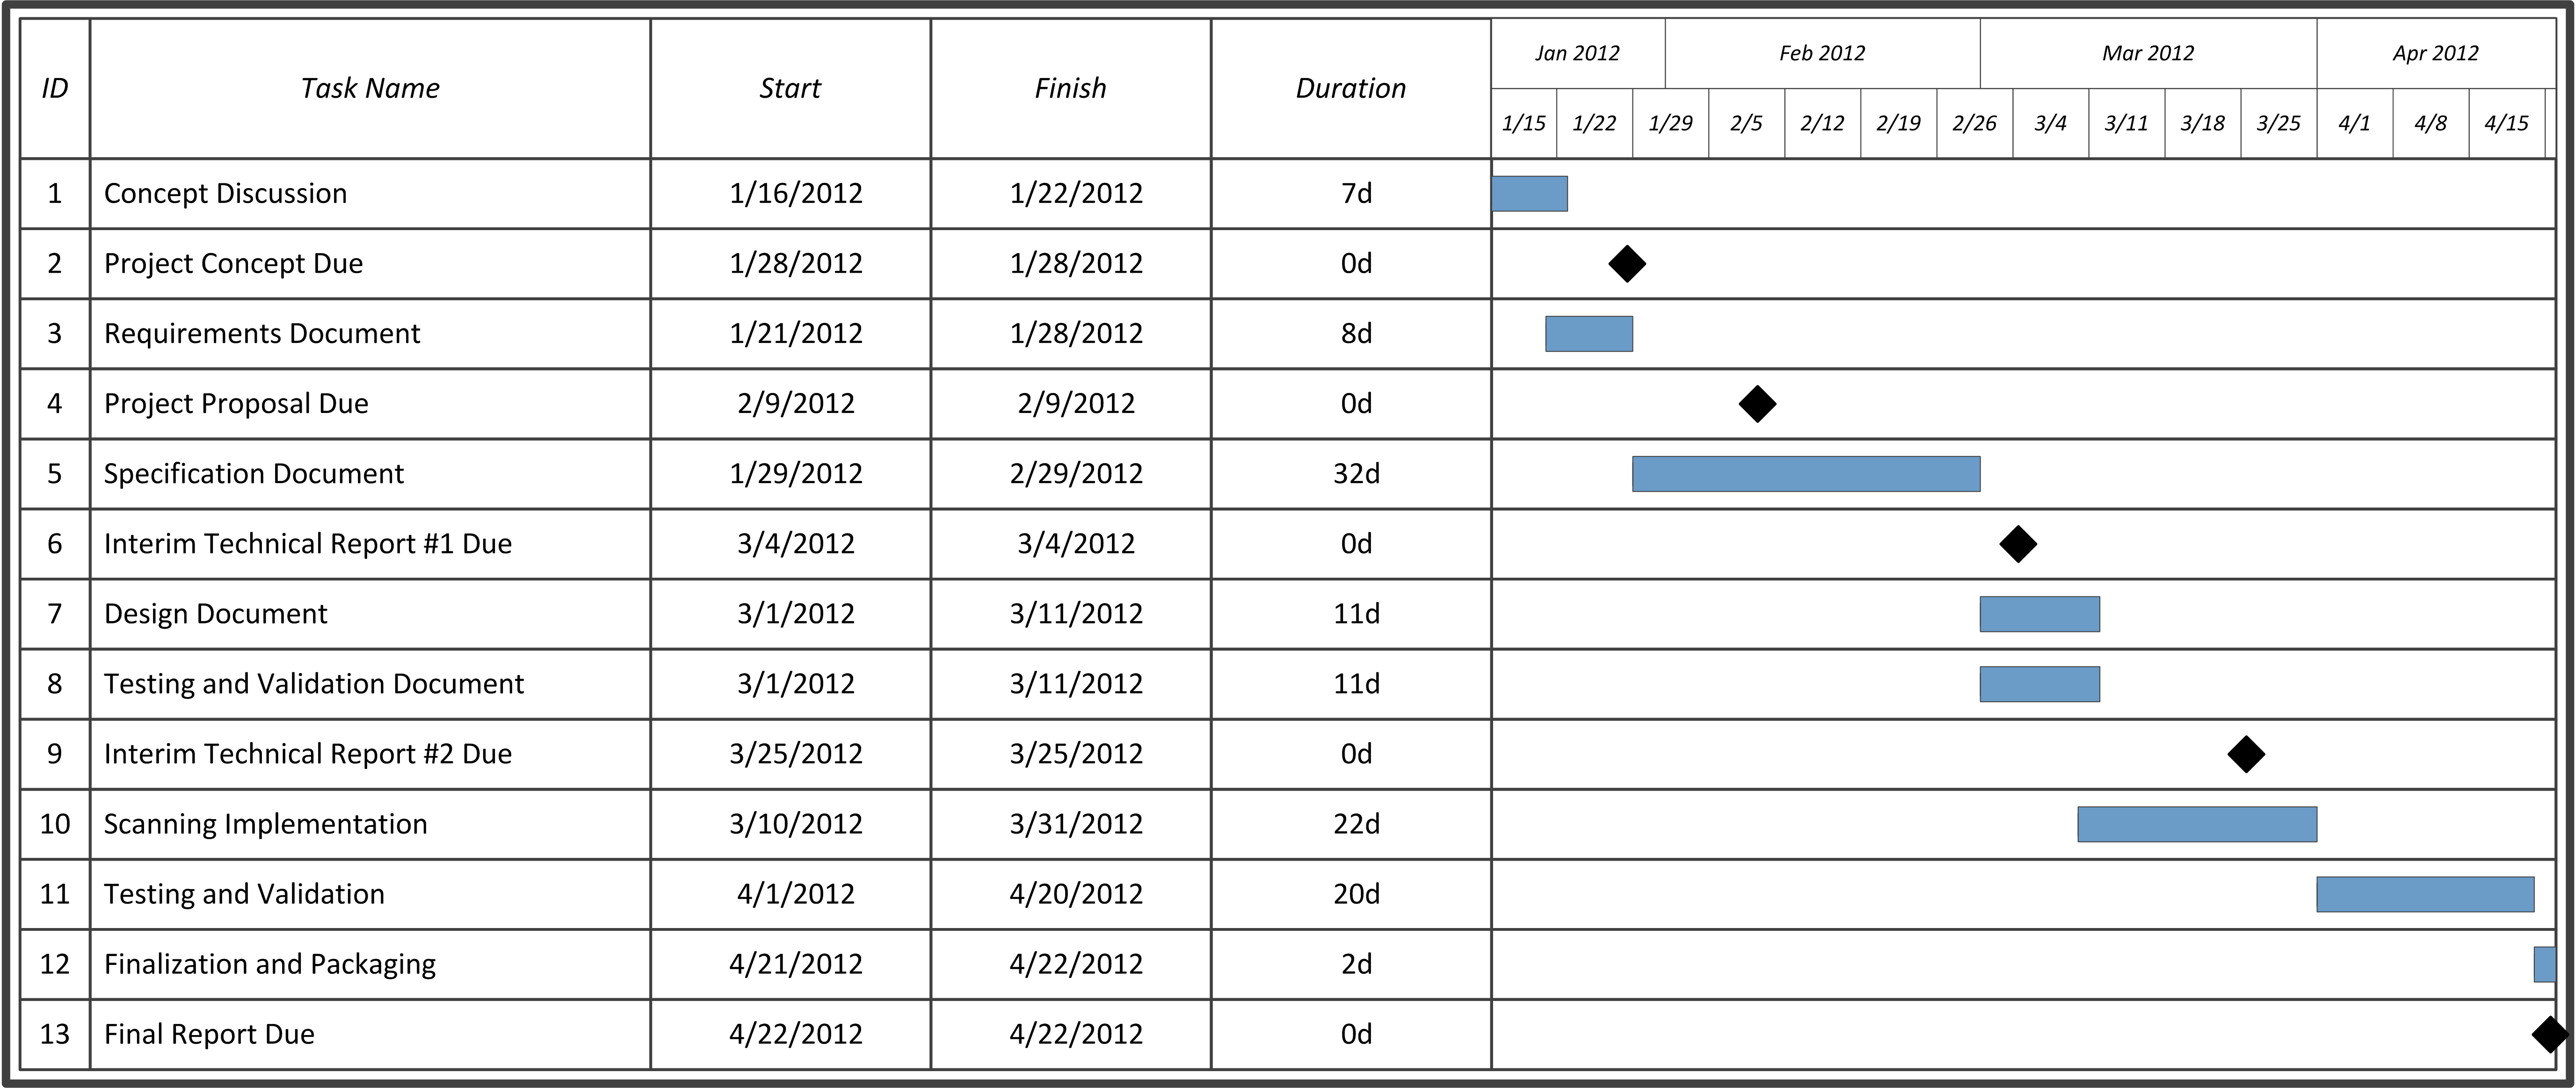
\includegraphics[scale=.7]{figures/GanttChart.png}
  	\caption{Gantt Chart}
  	\label{gantt}
\end{figure}

The project is on track according to the revised plan.  In the last report, it
was stated that the goal was to have a reasonable prototype in place by this
report.  This goal has been met, with two scanning sections entirely
implemented with more on the way.  At this point, since all of the scaffolding
is in place, there shouldn't be many more roadblocks in the way to finishing the
project on time.  Additionally, the project has been tested as development has
progressed, so the actual testing time shouldn't take nearly as long as stated
in the Gantt chart, so the implementation phase can get shifted back into the
testing phase if needed.  

The authors of this tool began by using pair programming at the beginning of the
project.  Once a good common ground had been established, the authors split off
work and began implementing separate scanning sections in a test driven
development method.  

\newpage



\section{Project Progress} \label{project_progress}
The authors have been making good progress on the project.  By spending almost
every waking hour for five days over spring break working on the project, a
substantial amount of code has been designed, implemented, and tested.  A large
amount of background ``scaffolding'' has been developed and added to the
project.  In this context, ``scaffolding'' refers to the common code that
practically all scan sections will need.  This includes, but is not limited to:

\begin{itemize}
  \item An easy runtime dynamic linker
  \item A wrapper around Win32 and NT error messages to convert them to C++
  exceptions
  \item A wrapper around Win32 Processes Handles
  \item A wrapper around Win32 File Handles
  \item A privilege granting wrapper
  \item Path manipulation functions
  \item String functions including escaping and unescaping
  \item Pre-defined output formats from the specification
  \item Whitelisting support
  \item A wrapper around the registry
  \item Rudimentary scripting, reordering, and execution
  \item Framework for developing and reporting progress back to user interfaces
  \item A wrapper around Win32 Service Control Manager 
\end{itemize}

This ``scaffolding'' is actually quite a large portion of the specifications
document \cite{Specification}.  In fact, these sections alone account for
sections two and three of the specification.

In addition to finishing these background scaffolding components, two scanning
sections have been completely implemented: running processes and installed
services and drivers.  It is important to note that while this is the only
user-facing progress that has been made, like at the last report, a significant
amount of background work is done and completed so that the features of the tool
can be implemented.  The authors expect scanning sections to be implemented more
quickly with the scaffolding largely out of the way.

The authors have also been testing and documenting the written code extensively.
At the time of this writing, there are at least two hundred unit tests written,
each making sure the above scaffolding components and scanning sections are
running properly.  There are also doxygen comments for all of the code so that
other developers can understand the source and contribute if they so desire.

Lastly, support for Windows 2000, Windows XP RTM, and Windows XP Service Pack 1
have been tentatively dropped. This is due to the use of Visual Studio 2010's
compiler, which cannot produce binaries for these operating systems.
The C runtime bundled with this compiler requires functions that were added to
Windows in Windows XP Service Pack 2.

This is stated as a ``tentative'' restriction because it is, in theory,
possible to mess with the build system enough to build binaries
for these operating systems, by providing our own implementations of the
missing functions.

However, at this point in time, it was decided that it is not worth the authors' time.
This is for a number of reasons, namely
that Microsoft is dropping support for these operating systems anyway and not
releasing security fixes anymore, so it doesn't make sense to attempt to clean
malware from these systems. 

There are some published workarounds that include replacement implementations of
these functions, but unfortuantely all such projects of which the authors are
aware are under the GNU General Public License (GPL). The authors do not wish
to release Instalog under the GPL, because a major goal of the project is to be
usable by both commercial and noncommercial software, which is not possible if
the project depends on GPL licensed code.

\newpage



\section{Discussion and Conclusions} \label{discussion}
At this point, we are both very proud of the project's progress.  We've
continued the momentum of ``doing it the right way'' since the last progress
report.  At the last report, we had written extensive documents explaining
exactly how the tool would work.  At this report, as mentioned in previous
sections, we have written a large amount of background code and tested it pretty
thoroughly on our machines.  While progress seems to be slow to people on the
outside of the project, we both know that we made considerable progress over
break and are very proud of the code we've written so far.

At this point, the benefits of good engineering practices are very evident.  The
detailed documents we wrote helped make the first steps towards creating an
implementation much less daunting because we knew exactly how the code would
work and has helped minimize confusion by keeping implementation separate from
project definition.  Test driven development has allowed us to modify, refactor,
and optimize the code and still make sure we didn't break anything.  

Overall, we have both enjoyed the time we've spent on this project.  This is one
of the first class projects we've worked on where the partner is helpful and
willing to put as much time in as the other.  The only thing that we dislike is
having to write formal design documents, but we realize that this is another
good engineering practice and will likely be helpful at some point in the
project's lifecycle.  

\newpage



\section{External Documents} \label{documents}
As of this writing, there are not currently any additional external documents
beyond the documents listed in section~\ref{design}.  By the final release of
the product, however, there will be a user's manual and programmer's manual that
will be included as external documents.  A list of third-party software use and
incorporation in the project will be included in the Design Document
\cite{Design}.

\newpage



\bibliography{ProjectReport}{} 
\bibliographystyle{plain}

\newpage



\appendix
\section{License} \label{license}
Instalog itself is to be released under the two clause form of the BSD license,
which is reprinted below:

\begin{verbatim}
Copyright © 2012, Jacob Snyder, Billy O'Neal III, and "sUBs"
All rights reserved.

Redistribution and use in source and binary forms, with or without
modification, are permitted provided that the following conditions are met: 

1. Redistributions of source code must retain the above copyright notice, this
   list of conditions and the following disclaimer. 
2. Redistributions in binary form must reproduce the above copyright notice,
   this list of conditions and the following disclaimer in the documentation
   and/or other materials provided with the distribution. 

THIS SOFTWARE IS PROVIDED BY THE COPYRIGHT HOLDERS AND CONTRIBUTORS "AS IS" AND
ANY EXPRESS OR IMPLIED WARRANTIES, INCLUDING, BUT NOT LIMITED TO, THE IMPLIED
WARRANTIES OF MERCHANTABILITY AND FITNESS FOR A PARTICULAR PURPOSE ARE
DISCLAIMED. IN NO EVENT SHALL THE COPYRIGHT OWNER OR CONTRIBUTORS BE LIABLE FOR
ANY DIRECT, INDIRECT, INCIDENTAL, SPECIAL, EXEMPLARY, OR CONSEQUENTIAL DAMAGES
(INCLUDING, BUT NOT LIMITED TO, PROCUREMENT OF SUBSTITUTE GOODS OR SERVICES;
LOSS OF USE, DATA, OR PROFITS; OR BUSINESS INTERRUPTION) HOWEVER CAUSED AND
ON ANY THEORY OF LIABILITY, WHETHER IN CONTRACT, STRICT LIABILITY, OR TORT
(INCLUDING NEGLIGENCE OR OTHERWISE) ARISING IN ANY WAY OUT OF THE USE OF THIS
SOFTWARE, EVEN IF ADVISED OF THE POSSIBILITY OF SUCH DAMAGE.
\end{verbatim}

This document, along with all other documentation related to Instalog,  is to be
released under the Creative Commons Attribution 3.0 Unported license. Human
readable and lawyer readable versions of this license can be found at
\url{http://creativecommons.org/licenses/by/3.0/}.

\newpage



\end{document}
